% MEMORY_DESIGN_REPORT_STATUS: final
\section{来源事实、人物条件与增量交付（11月2日）}
\label{sec:memory-design}
本轮固定原有340个片段记忆与65题，不重新生成感知或记忆。新增可追溯原文事实窗口、
显式人物条件软排序和前缀稳定的增量交付。S额外使用GPU BGE-M3构建的7965个
事实窗口旁路索引，按账号/视频/时间筛选并回源核对内容哈希；同时改为按实际
新增可见事实判断停搜。人物条件不等价于已核实的人脸/声音身份解析。
\begin{center}\small\begin{tabular}{lrrrr}\toprule
方案 & 有效回答 & 共同评分 & QA输入token & 调用\\\midrule
B：前次 balanced & 65/65 & 0.5923 & 4,804,362 & 365\\
B：前次独立重复 & 65/65 & 0.6000 & 4,707,523 & 361\\
M3-Agent 同模型参考适配 & 65/65 & 0.4615 & 569,796 & 310\\
F：原文事实窗口 & 65/65 & 0.5000 & 2,560,063 & 366\\
FI：事实 + 显式人物条件 & 65/65 & 0.4923 & 2,548,205 & 365\\
FIP：事实 + 人物 + 增量 & 64/65 & 0.5462 & 3,314,963 & 366\\
S：来源事实索引 + 增量修正 & 65/65 & 0.5846 & 3,456,572 & 369\\
S：独立重复 & 65/65 & 0.6077 & 3,408,547 & 365\\
B：本轮同期独立重复 & 65/65 & 0.5308 & 4,721,119 & 361\\
M3-Agent：本轮同记忆重复 & 65/65 & 0.4615 & 551,699 & 302\\
E：严格增量3500 + 收尾请求 & 65/65 & 0.5846 & 2,915,704 & 370\\
\bottomrule\end{tabular}\end{center}
同批评委共715条固定答案，seed=1102随机交错，不向评委发送方案名。
S独立运行两次的描述性均值为0.5962，同期B为0.5308。
这些是小规模开发集自动评分，不是人工准确率或官方M3-Agent复现。
全部消融、失败、逐题评分与用量见\code{experiments/m3_memory_design_20261102/REPORT.md}。
索引构建约63秒、37MB，QA用量不包含历史记忆生成。输入含缓存，
不能将输入token比例当成费用或端到端加速比。
\IfFileExists{figures/memory_design_tradeoff.pdf}{
\begin{figure}[htbp]\centering
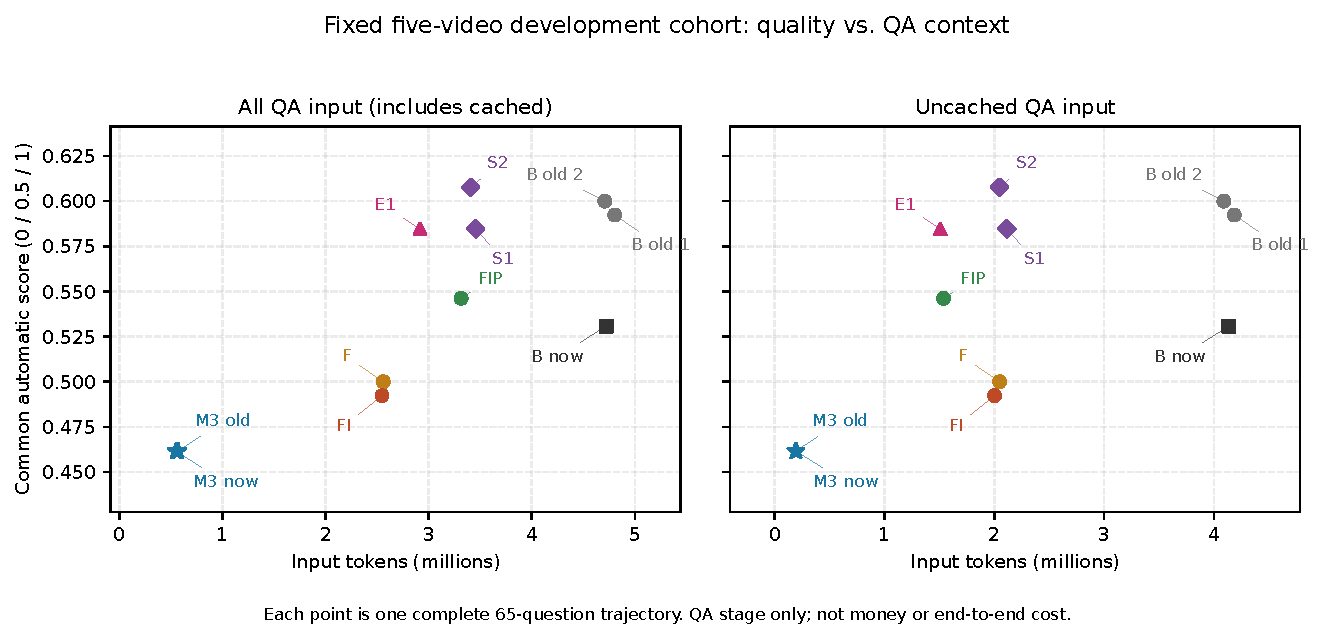
\includegraphics[width=\linewidth]{figures/memory_design_tradeoff.pdf}
\caption{同批自动评分与QA输入。每点为完整65题轨迹，重复运行分别显示；不是费用或端到端开销。}
\end{figure}}{}
实现及安全边界见\code{docs/m3_memory_design.md}。
\subsection{五视频结果}
S为两次轨迹的分视频平均，M3为原轨迹与本轮重复的平均；重复不增加独立题数。
\begin{center}\small\begin{tabular}{lrrrrr}\toprule
视频 & 题数 & B同期 & S均值 & E & M3均值\\\midrule
\code{study_05} & 12 & 0.4167 & 0.4583 & 0.4583 & 0.4583\\
\code{gym_03} & 11 & 0.6818 & 0.6591 & 0.6364 & 0.6364\\
\code{bedroom_04} & 11 & 0.7273 & 0.7955 & 0.7727 & 0.6364\\
\code{study_18} & 14 & 0.3214 & 0.4286 & 0.4643 & 0.2679\\
\code{kitchen_20} & 17 & 0.5588 & 0.6618 & 0.6176 & 0.3971\\
\bottomrule\end{tabular}\end{center}
例如E在gym\_03低于同期B，不能宣称每个视频都提升；study\_18仍是短板。
\subsection{按数据集类别的诊断}
类别为数据集多标签，同一道题可属于多个类别，不能相加当作总分。
多跳推理只有1题，不作能力泛化判断。以下仍是同批自动评分。
\begin{center}\small\begin{tabular}{lrrrrr}\toprule
方案 & 人物理解(21) & 跨模态推理(21) & 多细节推理(28) & 知识提取(25) & 多跳推理(1)\\\midrule
M3同期重复 & 0.643 & 0.452 & 0.393 & 0.440 & 0.500\\
B同期 & 0.833 & 0.548 & 0.429 & 0.420 & 1.000\\
S首次 & 0.857 & 0.667 & 0.518 & 0.460 & 1.000\\
S重复 & 0.881 & 0.643 & 0.464 & 0.600 & 1.000\\
E首次 & 0.881 & 0.571 & 0.518 & 0.480 & 0.500\\
\bottomrule\end{tabular}\end{center}
